\chapter{Introduction}
\label{chp:introduction} 

Introduction
\section{About the Thesis}

\subsection{Long Term Goal and Previous Work}

\subsubsection{The Topic - Mobile Autonomous Robot}

The robot system that was used in this project, has been developed over the course of many preceding master and specialization projects. The long term goal of these projects is to develop a mobile autonomous robot for maintenance and inspection on topside offshore installations. The topic is given by Professor Tor Onshus at \ac{ITK}. A description of this topic\footnote{\url{http://folk.ntnu.no/onshus/Oppgaver.htm}}, suggests some possible applications for such a robot: 

\begin{itemize}
	\item The robot could serve in a supporting role as a part of \ac{IO}.
	\item It can also be used to prepare an unmanned topside offshore installation before the arrival of a maintenance crew, by performing safety checks and preparing the helicopter landing pad.  
	\item Allow personnel to perform remote inspection and maintenance through telepresence.
	\item  In combination with \ac{VR}, the robot could be used for training purposes. 
\end{itemize}



\subsubsection{Building the Mobile Platform}

\subsubsection{Simultanious Localization and Mapping}

\section{Implementation Overview}

\begin{figure}[p]
	\centering
	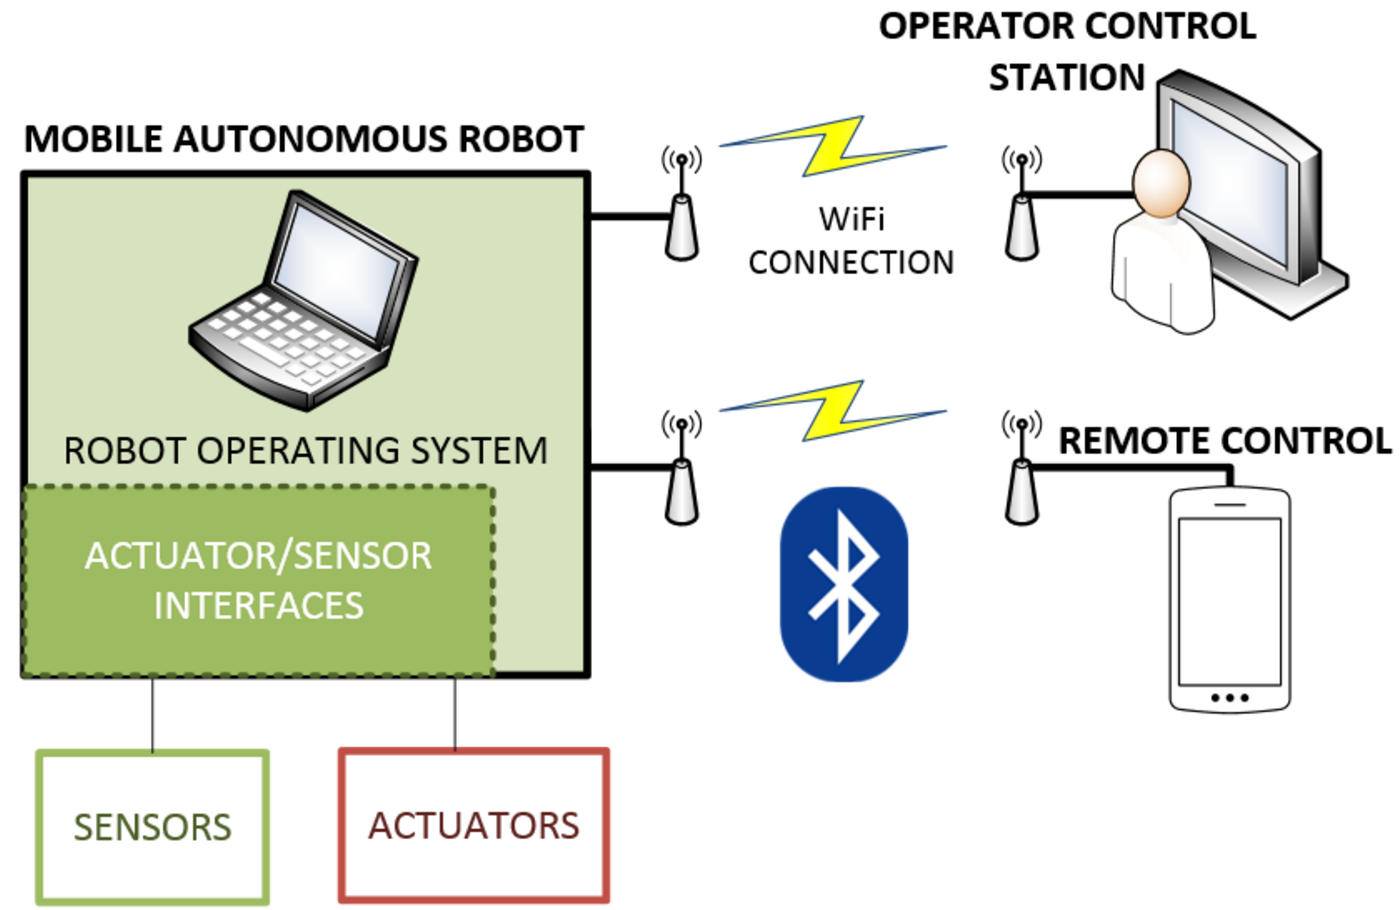
\includegraphics[width=0.8\textwidth]{conseptDrawing}
	\caption{System Concept. }
	\label{fig:conseptDrawing}
\end{figure}

\section{Thesis Structure}